\documentclass[11pt]{article}
\usepackage{amsmath}
\usepackage{physics}
\usepackage{amssymb}
\usepackage{graphicx}
\usepackage{hyperref}
\usepackage{amsfonts}
\usepackage{cancel}
\usepackage{xcolor}
\hypersetup{
	colorlinks,
	linkcolor={black!50!black},
	citecolor={blue!50!black},
	urlcolor={blue!80!black}
}
\newcommand{\f}[2]{\frac{#1}{#2}}
\usepackage{newpxtext,newpxmath}
\usepackage[left=1in,right=1in,top=1.25in,bottom=1.25in]{geometry}
\usepackage{framed}
\usepackage{enumerate}

\usepackage{caption}
\usepackage{subcaption}

%\newcommand{\fig}[1]{figure #1}
%\newcommand{\explain}{appendix?}
%\newcommand{\rat}{\mathbb{Q}}
%
%\newcommand{\mathbb{R}}{\mathbb{R}}
%\newcommand{\nat}{\mathbb{N}}
%\newcommand{\inte}{\mathbb{Z}}
%\newcommand{\M}{{\cal{M}}}
%\newcommand{\sss}{{\cal{S}}}
%\newcommand{\rrr}{{\cal{R}}}
%\newcommand{\uu}{2pt}
%\newcommand{\vv}{\vec{v}}
%\newcommand{\comp}{\mathbb{C}}
%\newcommand{\field}{\mathbb{F}}
%\newcommand{\f}[1]{ \hspace{.1in} (#1) }
%\newcommand{\set}[2]{\mbox{$\left\{ \left. #1 \hspace{3pt}
%\right| #2 \hspace{3pt} \right\}$}}
%\newcommand{\integral}[2]{\int_{#1}^{#2}}
%\newcommand{\ba}{\hookrightarrow}
%\newcommand{\ep}{\varepsilon}
%\newcommand{\limit}{\operatornamewithlimits{limit}}
%\newcommand{\ddd}{.1in}
%\newcommand{\ccc}{2in}
%\newcommand{\aaa}{1.5in}
%\newcommand{\B}{{\cal B}}
%\newcommand{\C}{{\cal C}}
%\newcommand{\D}{{\cal D}}
%\newcommand{\FF}{{\cal F}}
\usepackage{amssymb}% http://ctan.org/pkg/amssymb
\usepackage{pifont}% http://ctan.org/pkg/pifont
\newcommand{\cmark}{\ding{51}}%
\newcommand{\xmark}{\ding{55}}%
\newcommand{\p}{\partial}%
%\usepackage{MnSymbol,wasysym}



\usepackage{listings}
\captionsetup[lstlisting]{margin=0cm,format=hang,font=small,format=plain,labelfont={bf,up},textfont={it}}
\renewcommand*{\lstlistingname}{Code \textcolor{violet}{\textsl{Mathematica}}}
\definecolor{gris245}{RGB}{245,245,245}
\definecolor{olive}{RGB}{50,140,50}
\definecolor{brun}{RGB}{175,100,80}
\lstset{
	tabsize=4,
	frame=single,
	language=mathematica,
	basicstyle=\scriptsize\ttfamily,
	keywordstyle=\color{black},
	backgroundcolor=\color{gris245},
	commentstyle=\color{gray},
	showstringspaces=false,
	emph={
		r1,
		r2,
		epsilon,epsilon_,
		Newton,Newton_
	},emphstyle={\color{olive}},
	emph={[2]
		L,
		CouleurCourbe,
		PotentielEffectif,
		IdCourbe,
		Courbe
	},emphstyle={[2]\color{blue}},
	emph={[3]r,r_,n,n_},emphstyle={[3]\color{magenta}}
}






\begin{document}
\begin{center}
{\large \bf PH312: Physics of Fluids (Prof. McCoy) -- Reflection}\\
{ Huan Q. Bui}\\
April 2, 2021
\end{center}



\noindent \textbf{1.} Purcell really stressed how, for microbial animals, inertia doesn't really matter because the fluid, relative to their size and speed, is too viscous/thick to \textit{swim}. What does it mean to swim, anyway? If you put someone in a pool of molasses and the person tries to wiggle their way through the fluid, you wouldn't call it \textit{swimming}, would you? From here, Purcell talked about \textit{reciprocal motion} in swimming and emphasized that this kind of motion gets you nowhere when Re is too small (since the viscous term in the NS equation goes away and all that's left is the diffusion term). This is the Scallop Theorem. He then moved on to talk about various swimming mechanisms at low Re. \\



\noindent \textbf{2.} We want to show that the strength of a vortex tube does not depend on the choice of $C$ and $A$. To do this, we pick two curves $C_1$ and $C_2$ and calculate the circulation for each curve in two ways using Stokes' theorem. 
\begin{equation*}
\Gamma_i = \oint_{C_i} \mathbf{u}\cdot d\mathbf{l} = \int_{A_i} \boldsymbol{\omega} \cdot d \mathbf{S}
\end{equation*}
Here, $A_1$ and $A_2$ are the ends of a vortex tube. \\


We know that $\nabla \cdot  \boldsymbol{\omega} = 0$, and so 
\begin{equation*}
\oint_A \boldsymbol{\omega} \cdot d\mathbf{S} = 0
\end{equation*}
where $\oint_A$ is the integral over the entire area of a tube.  By definition, the normal vector to the side of the tube is perpendicular to the vortex lines, so the contribution from the sides is zero. So, this means that the contribution from the $A_1$ and $A_2$ integrals (whose orientations are pointing out of the tubes) are opposite and equal, and so, along the direction of vortex lines, we have
\begin{equation*}
\int_{A_1} \boldsymbol{\omega} \cdot d \mathbf{S}
=
\int_{A_2} \boldsymbol{\omega} \cdot d \mathbf{S},
\end{equation*} 
i.e., $\Gamma_1 = \Gamma_2 = \Gamma$, a constant, since the loops $C_1, C_2$ are arbitrary. \\



\noindent \textbf{3.}  The flow is axisymmetric emanating from a point source $Q$. Since the source has no preferred axis of symmetry, the axisymmetry implies spherical symmetry. So, $u_\theta = u_\varphi = 0$. Now, by Gauss' law, we know that the total flow through a sphere of radius $r$ centered at the source, $Q$, is equal to the flux integral over the surface of the sphere $\oint_S \mathbf{u}\cdot d\mathbf{S} = u_r\times (4\pi r^2)$ due to spherical symmetry. This leaves us with $u_r = Q/4\pi r^2$. \footnote{We note that Gauss' law here is just a another way to state the continuity equation.} \\

\noindent Since $0 = u_\theta \propto \p_r \psi$, the streamfunction $\psi$ has no $r$-dependence (and of course, no $\varphi$-dependence either). So, $\psi = \psi(\theta)$ is given by 
\begin{equation*}
\p_r \psi = u_r r^2 \sin\theta = \f{Q}{4\pi} \implies \psi(\theta) = -\f{Q}{4\pi}\cos\theta.
\end{equation*}
We see that since $u_\varphi = u_\theta = 0$ and that $u_r$ has no $\varphi$- nor $\theta$-dependence, the curl of $\mathbf{u}$ is zero, and so $\mathbf{u}$ is irrotational. Alternatively, we see that $\mathbf{u}$ is the gradient of the \textit{potential flow} function $\phi = -Q/4\pi r$, and so it must have zero curl. \\





\noindent \textbf{4.} 
\begin{enumerate}[(a)]
	\item With $\psi = Ur^2\sin^2\theta/2$, we have $u_r = U\cos\theta$ and $u_\theta = -U\sin\theta$. With $\varphi = 0$, we see that 	
	$\mathbf{u} = U\cos\theta \hat{r} - U\sin\theta \hat{\theta} = U \hat{x}$. so, the flow field is uniform along $x$ with strength $U$. 
	
	
	\item To make things easier, let us set $m=1$. With $\psi = -m\sin^2\theta/r$, we can find $\mathbf{u}$ in spherical coordinates using the definition of $u_i$ in terms of $\psi$. Then, to plot things in Mathematica we will need to convert $\mathbf{u}$ into Cartesian coordinates. All of this can be done in code:
	\begin{lstlisting}
	\[Psi][r_,\[Theta]_]:=-(1/r)*Sin[\[Theta]]^2;
	Ur[r_,\[Theta]_]:=(1/(r^2*Sin[\[Theta]]))*D[\[Psi][r,\[Theta]],\[Theta]];
	UThe[r_,\[Theta]_]:=(-1/(r*Sin[\[Theta]]))*D[\[Psi][r,\[Theta]],r];
	
	TransformedField[ 
	"Spherical" -> "Cartesian", {Ur[r,\[Theta]],UThe[r,\[Theta]],0},  
	{r, \[Theta],\[Phi]} -> {x,y,z}] // Simplify
	\end{lstlisting}
	
	We find that, in Cartesian coordinates,
	\begin{equation*}
	\mathbf{u} = \f{1}{(x^2+y^2+z^2)^{5/2}}\left( -3xz, -3yz, x^2+y^2-2z^2 \right). 
	\end{equation*}
	We can look at the streamlines in 3D, but of course since there is the $z$-symmetry, we can just set $y=0$ and look in the $xz$-plane. 
	\begin{figure}[!htb]
		\centering
		\begin{subfigure}{0.49\textwidth}
			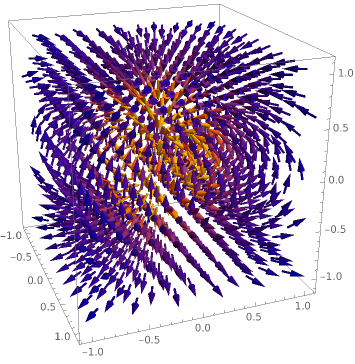
\includegraphics[scale=0.5]{stream3D}
		\end{subfigure}
		\begin{subfigure}{0.49\textwidth}
			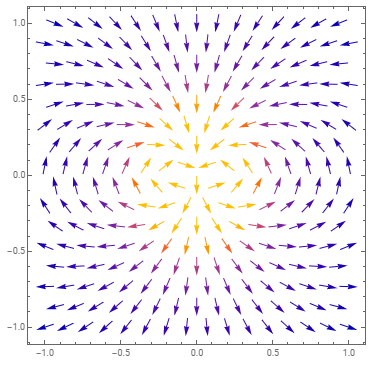
\includegraphics[scale=0.6]{stream2D}
		\end{subfigure}
	\end{figure}
	The streamlines look like the electric field lines due to a dipole in electrostatics. 
	
	
	
	\item $\phi = U r \cos\theta$ is the potential function for the uniform flow since $\mathbf{u} = \nabla \phi = U(\cos\theta, -\sin\theta,0)$ in spherical coordinates, which is $(U,0,0)$ in Cartesian coordinates. This says that $\mathbf{u}$ is a uniform flow field of strength $U$ in the $x$-direction. Here, the gradient in spherical coordinates is found by 
	\begin{lstlisting}
	Grad[U*r*Cos[\[Theta]],{r,\[Theta],\[Phi]}, "Spherical"]
	\end{lstlisting}
	
	Similarly, for $\phi = m\cos\theta/r^2$, we find $\mathbf{u} = \nabla \phi = (-2m\cos\theta/r^3, -m\sin\theta/r^3,0)$ in spherical coordinates. Converting this back to Cartesian coordinates we find the same answer we found in (b), which is $\mathbf{u} = m(-3xz,-3yz, (x^2+y^2-2z^2) )/(x^2+y^2+z^2)^{5/2}$.
	\begin{lstlisting}
	Grad[(m/r^2)*Cos[\[Theta]],{r,\[Theta],\[Phi]}, "Spherical"]
	
	TransformedField[ 
	"Spherical" -> "Cartesian", {-2 m Cos[\[Theta]]/r^3, -m*Sin[\[Theta]]/r^3 ,0} , 
	{r, \[Theta],\[Phi]} -> {x,y,z}] // Simplify
	\end{lstlisting}
	
\end{enumerate}



\noindent \textbf{5.} 
\begin{enumerate}[(a)]
	\item The irrotational flow around a sphere or radius is a vector sum of the uniform flow field far from the sphere and the axisymmetric flow near the field. This simply corresponds to a scalar (weighted) sum of the streamfunctions associated with each flow profile. \\
	
	
	To see why this flow is irrotational, we can refer back to the preceding problems. The uniform flow in one direction is clearly irrotational. The doublet flow is also irrotational because it can be described by a potential flow. Finally, the curl is linear, so adding two irrotational fields gives an irrotational field. \\
	

	Imposing the no-slip condition at $r=a$, we have $\psi(r=a) = 0$ for all $\theta$. This holds only if $a = (2m/U)^{1/3}$, and so $\boxed{m = U a^3/2}$. Alternatively,  we can obtain the same answer by setting  the associated velocity components:
	\begin{equation*}
	u_r = \f{1}{r^2\sin\theta}\p_\theta \psi = \left(  U-\f{2m}{r^3} \right) \cos\theta
	\end{equation*}
	and 
	\begin{equation*}
	u_\theta = -\f{1}{r\sin\theta}\p_r\psi = -\left(U + \f{m}{r^3} \right)\sin\theta
	\end{equation*}
	to zero at $r=a$ and solve for $m$. 
	
	
	\item The Euler equation says that $(\mathbf{u}\cdot \nabla)\mathbf{u} = -(1/\rho)\nabla p$. From the appendix, we find that
	\begin{equation*}
	\mathbf{u}\cdot \nabla  = u_r \p_r + \f{1}{r}u_\theta \p_\theta + \cancel{\f{u_\varphi}{r\sin\theta} \p_\varphi} = u_r \p_r + \f{1}{r}u_\theta \p_\theta
	\end{equation*}
	Applying this to $\mathbf{u}$, we find 
	\begin{equation*}
	-\f{1}{\rho}\nabla p = \left\{
	 \frac{U^2\left(r^3-a^3\right)\left(6a^3\cos^2\theta+\left(a^3+2r^3\right)\sin^2\theta\right)}{2r^7}, \frac{U^2\left(10a^3r^3-5a^6+4r^6\right)\sin(2\theta)}{8r^7} , 0
	\right\}
	\end{equation*}
	Here's the Mathematica code to calculate this:
	\begin{lstlisting}
	(U*( 1 -a^3/r^3)* Cos[\[Theta]])*D[U*( 1 -a^3/r^3)* Cos[\[Theta]],r]
	+(1/r)*(-U*( 1 + (1/2)*a^3/r^3 )* Sin[\[Theta]])*D[U*( 1 -a^3/r^3)* Cos[\[Theta]]
	,\[Theta]]//Simplify
	
	(U*( 1 -a^3/r^3)* Cos[\[Theta]])*D[ -U*( 1 + (1/2)*a^3/r^3 )* Sin[\[Theta]],r]
	+(1/r)*(-U*( 1 + (1/2)*a^3/r^3 )* Sin[\[Theta]])*D[ -U*( 1 
	+ (1/2)*a^3/r^3 )*Sin[\[Theta]],\[Theta]]//Simplify
	\end{lstlisting}
	
	Now, the spherical gradient tells us that $\p_r p$ is the first component of the vector above. So, we integrate this component over $r$ and set $r=a$ to find the contribution to $p-p_\infty$ at $r=a$. It turns out that this part is zero (or constant, since we can always perform a gauge transformation with $p_\infty$). The Mathematica code to do this is:
	\begin{lstlisting}
	FirstComponent[r_,\[Theta]_] := (-a^3+r^3)*U^2*(6a^3Cos[\[Theta]]^2
	 +(a^3 + 2r^3)*Sin[\[Theta]]^2)/(2r^7) ;
	
	R[r_] := Integrate[ FirstComponent[r,\[Theta]], r]//Simplify
	
	R[a]
	>> 0
	\end{lstlisting}
	
	
	
	Next, we look at the contribution from the second component. The spherical gradient tells us that this component is equal to $(1/r)\p_\theta p$. So, we integrate this component over $\theta$ and multiply it by $r$. Once this is done, we set $r=a$ and evaluate:
	
	\begin{lstlisting}
	SecondComponent[r_,\[Theta]_] := U^2(10a^3r^3-5a^6+4r^6)*Sin[2\[Theta]]/(8r^7);
	
	Theta[r_] := r*Integrate[ SecondComponent[r,\[Theta]], r]//Simplify
	
	Theta[a]
	>> -(9/16)*U^2*Cos[2\[Theta]]
	\end{lstlisting}
	
	We find that 
	\begin{equation*}
	p-p_\infty = -\rho \left( -\f{9}{16} U^2 \cos(2\theta) \right) = \f{1}{2} \rho U^2 \times \f{9}{8}\left(1 -2\sin^2\theta \right).
	\end{equation*}
	where we have used $\cos(2\theta) = 1 - 2\sin^2\theta$. Now, re-adjusting the pressure at infinity (it doesn't really matter what constant value $p_\infty$ takes) we can obtain the given expression:
	\begin{equation*}
	\boxed{p - p_\infty = \f{1}{2}\rho U^2 \left( 1- \f{9}{4}\sin^2\theta \right)}
	\end{equation*}
	\textcolor{blue}{I think this re-adjustment is done so that at $\theta =0$, we have $p-p_\infty = \rho U^2/2$, which aligns more nicely with Bernoulli's equation.}\\
	
	
	We see that this pressure field is front-back symmetrical, so there is \textbf{zero} drag implied.  
	

\end{enumerate}



\end{document}




